\documentclass{article}

\usepackage{graphicx}
\usepackage{tikz}
\usepackage{tikzsymbols}
\usetikzlibrary{calc,patterns,shapes.geometric}
\pagestyle{empty}
\usepackage[margin=0pt]{geometry}
\geometry{papersize={14in,12in}}

\def\centerarc[#1](#2)(#3:#4:#5){\draw[#1] ($(#2)+({#5*cos(#3)},{#5*sin(#3)})$) arc (#3:#4:#5);}

\begin{document}
	\begin{figure}
		\centering
		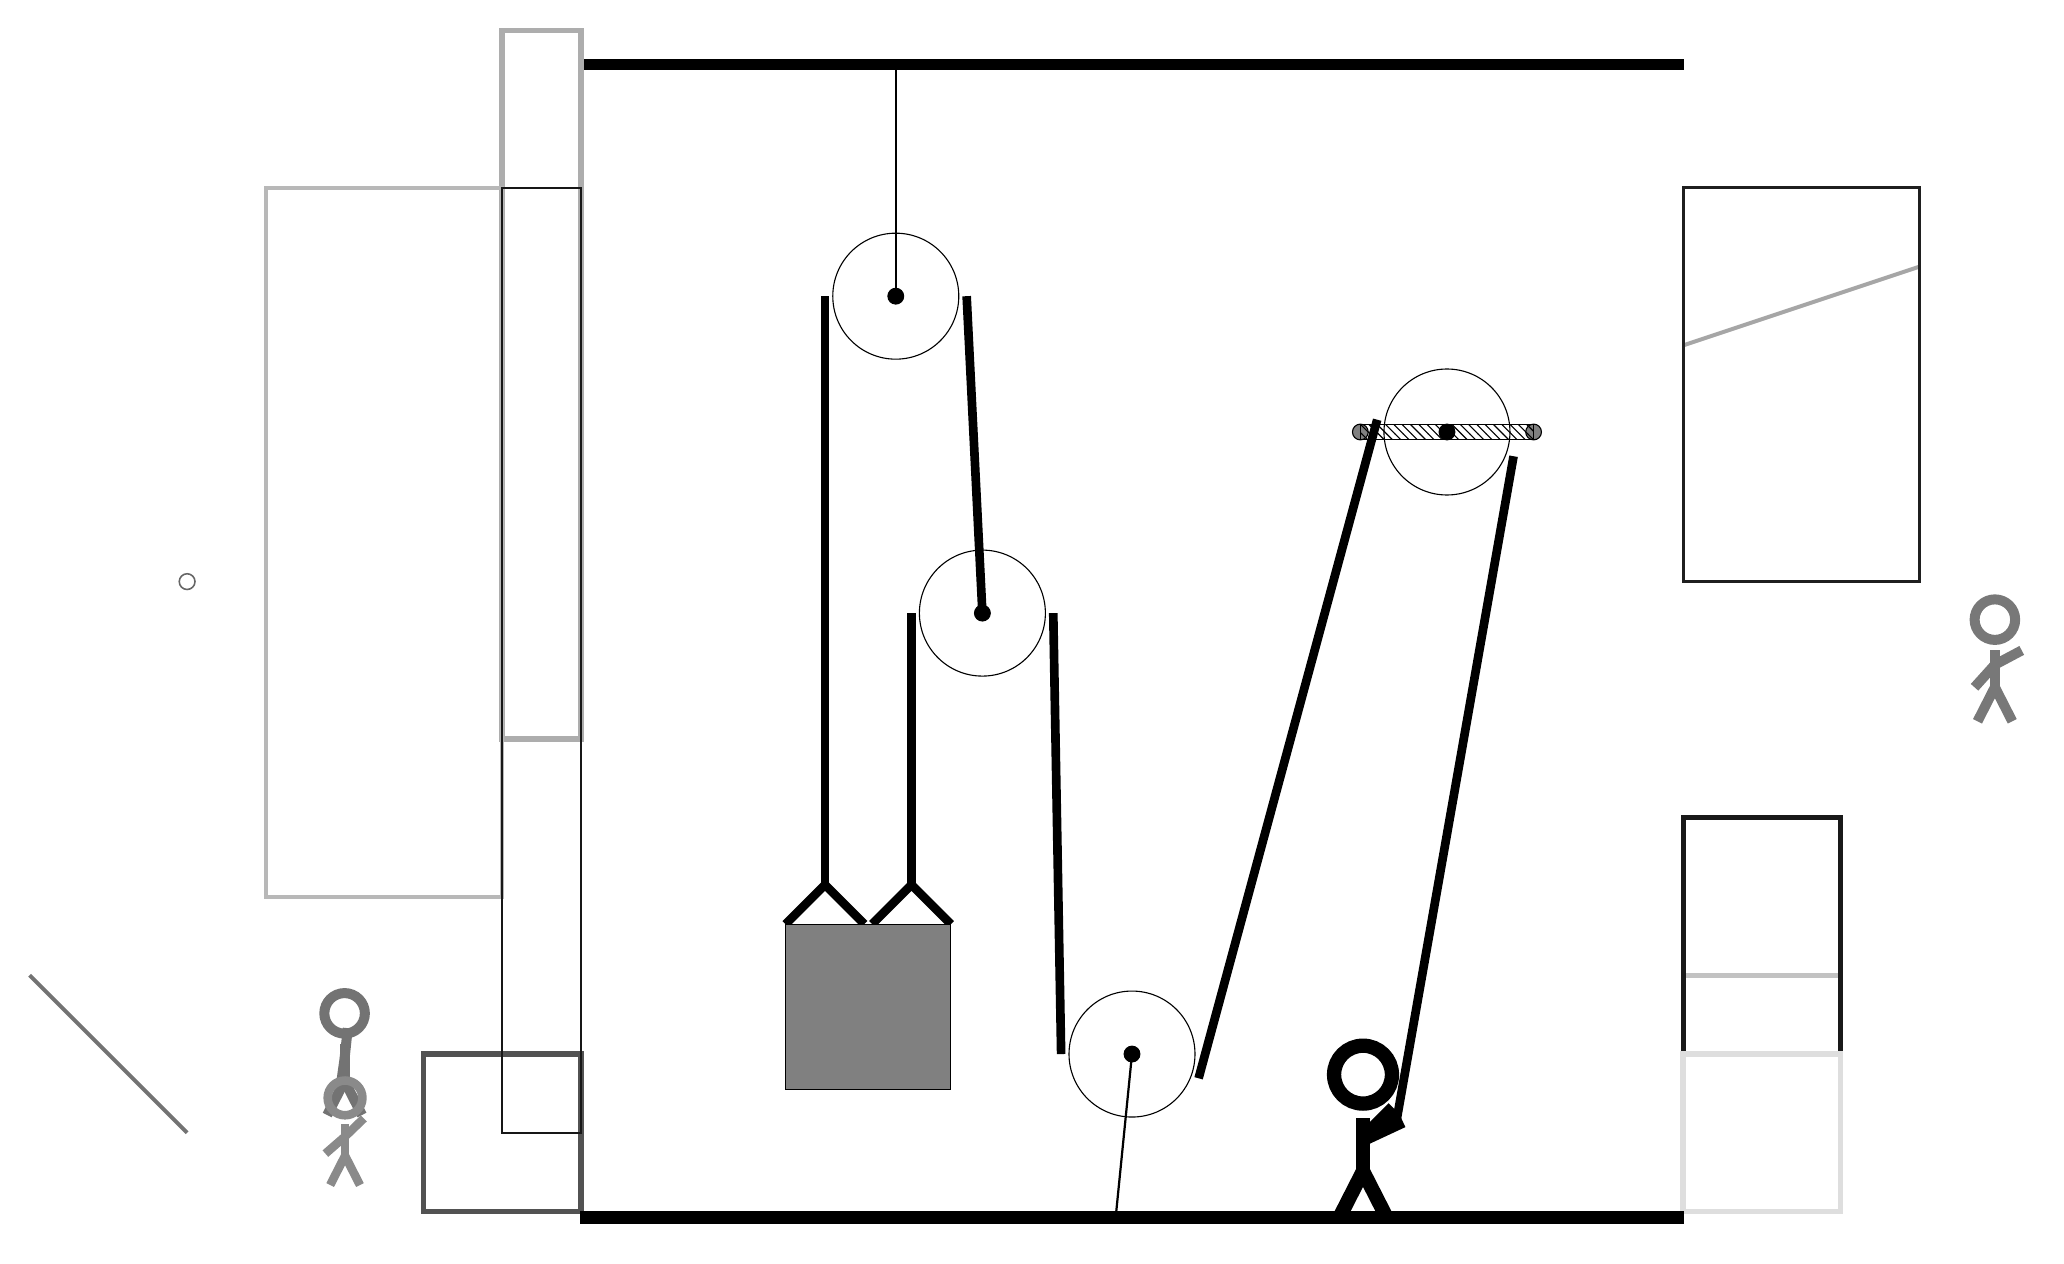
\begin{tikzpicture}
			%%%%% START %%%%%
			
			\draw[fill=black] (-2, 11.5) rectangle (12, 11.625);
			
			\draw (2, 8.625) circle (0.8);
			\draw[fill=black] (2, 8.625) circle (0.1);
			\draw[thick] (2, 8.625) -- (2, 11.5);
			
			\draw (3.1, 4.6) circle (0.8);
			\draw[fill=black] (3.1, 4.6) circle (0.1);
			
			\draw (5, -1) circle (0.8);
			\draw[fill=black] (5, -1) circle (0.1);
			\draw[thick] (5, -1) -- (4.8, -3);
			
			\draw[line width=0.7mm, color=black!32] (-3, 12) rectangle (-2, 3);
			
			\draw[line width=0.7mm, color=black!68] (-2, -3) rectangle (-4, -1);
			\draw[line width=0.6mm, color=black!24] (12, 0) rectangle (14, 0);
			\node[line width=0.2mm, color=black!53] at (16, 4) {\Strichmaxerl[7][48][28]};
			\draw[line width=0.5mm, color=black!55](-7, -2) -- (-9, 0);
			
			\node[line width=0.6mm, color=black!55] at (-5, -1) {\Strichmaxerl[7][82][84]};
			\draw[line width=0.5mm, color=black!35](12, 8) -- (15, 9);
			\draw[line width=0.5mm, color=black!28] (-3, 10) rectangle (-6, 1);
			\draw[line width=0.4mm, color=black!88] (12, 5) rectangle (15, 10);
			\draw[line width=0.2mm, color=black!91] (-2, 10) rectangle (-3, -2);
			
			\node[line width=0.5mm, color=black!46] at (-5, -2) {\Strichmaxerl[6][41][44]};
			\draw[line width=0.6mm, color=black!90] (12, 2) rectangle (14, -1);
			\draw[line width=0.7mm, color=black!13] (14, -1) rectangle (12, -3);
			
			\draw [line width=0.2mm, color=black!60](-7, 5) circle (0.1);
			
			\draw (9, 6.9) circle (0.8);
			\draw[fill=black] (9, 6.9) circle (0.1);
			\draw[fill=black!50] (7.9, 6.9) circle (0.1);
			\draw[fill=black!50] (10.1, 6.9) circle (0.1);
			\draw[pattern=north west lines, pattern color=black] (7.9, 7.0) rectangle (10.1, 6.8);
			
			\draw[line width = 1.1mm]  (0.6, 0.65) -- (1.1, 1.15) -- (1.6, 0.65);
			\draw[line width = 1.1mm]  (1.7, 0.65) -- (2.2, 1.15) -- (2.7, 0.65);
			\draw[fill=black!50] (0.6, 0.65) rectangle (2.7, -1.45);
			
			\draw[line width = 1.1mm] (1.1, 8.625) -- (1.1, 1.15);
			\centerarc[line width = 1.1mm](2, 8.625)(0:180:0.9);
			\draw[line width = 1.1mm] (2.9, 8.625) -- (3.1, 4.6);
			\draw[line width = 1.1mm] (2.2, 4.6) -- (2.2, 1.15);
			\centerarc[line width = 1.1mm](3.1, 4.6)(0:180:0.9);
			\draw[line width = 1.1mm] (4.0, 4.6) -- (4.1, -1);
			\centerarc[line width = 1.1mm](5, -1)(180:340:0.9);
			\draw[line width=1.1mm](5.8457, -1.3078) -- (8.1137, 7.0562);
			\centerarc[line width = 1.1mm](9, 6.9)(-20:170:0.9);
			\draw[line width=1.1mm](9.8457, 6.5922) --  (8.35, -1.9);
			
			\node at (8, -2) {\Strichmaxerl[10][225][25]};
			
			\draw[fill=black] (-2, -3) rectangle (12, -3.15);
			
			%%%%% END %%%%%
		\end{tikzpicture}
	\end{figure}	
\end{document}